\documentclass[9pt]{beamer}
\usetheme{cmepda}

\usepackage[utf8]{inputenc}
\usepackage[T1]{fontenc}


\title{\scriptsize Computing Methods for Experimental Physics and Data Analysis}
\subtitle{Introduction}
\date{\today}
\author{L.~Baldini, F.~A.~Di Bello, G.~Lamanna, F.~Lizzi, A.~Manfreda, A.~Retico, A.~Rizzi}
\institute[UNIPI and INFN]{Universit\`a and INFN--Pisa}
\email{luca.baldini@pi.infn.it}


\begin{document}


\titleframe

\begin{frame}
  \frametitle{Goals and prerequisites}
  \begin{itemize}
  \item What is this all about?
    \begin{itemize}
    \item Collaborative code development and best practices
    \item Python basics, standard library and scientific ecosystem
    \item Algorithms and data structures
    \item Machine learning
    \item Specific tools for high-energy physics or medical physics
    \end{itemize}
  \item \alert{This is not so much about Python or C++---it is about how to
    write code for effective data analysis}
  \item Will I be a professional data scientist at the end of the semester?
    \begin{itemize}
    \item No, but hopefully you'll be able to poke around and find the right
      tool for the job at hand
    \end{itemize}
  \item Pre-requisites
    \begin{itemize}
    \item Have a vague idea of how a computer operates
    \item If you have ever programmed before that would be great!
    \item \alert{We shall ask you to fill a form next week to gauge your
      background and expectations}
    \end{itemize}
  \end{itemize}
\end{frame}


\begin{frame}
  \frametitle{Basic structure of the course}
  \begin{cmepdapicture}
    \pgfmathsetmacro{\y}{0.90}
    \pgfmathsetmacro{\dy}{0.135}
    \pgfmathsetmacro{\mw}{90pt}
    \node[cmepdadiagblock, name=basic, minimum width=\mw] at (0.5, \y) {
      Basic module\\[2pt] 5~weeks: Sep~16--Oct~21
    };
    \node[cmepdadiagblock, name=advanced, minimum width=\mw] at (0.5, \y-\dy) {
      Advanced module\\[2pt] 5~weeks: Oct~24--Nov~25
    };

    \node[draw, fit=(basic)(advanced), inner sep=10pt, rounded corners,
      style=dashed, line width=0.6pt] (base) {};
    \node [right=0pt of base.east, anchor=west] {6~CFU (mandatory for MS)};

    \node[cmepdadiagblock, name=ml, minimum width=\mw] at (0.15, \y-2.75*\dy) {
      Machine Learning\\[2pt] 5~weeks: Nov 28--Mar~2026
    };

    \node[cmepdadiagblock, name=hep, minimum width=\mw] at (0.5, \y-3.5*\dy) {
      High-Energy Physics\\[2pt] 5~weeks: Mar--Apr~2026
    };
    \node[cmepdadiagblock, name=med, minimum width=\mw] at (0.85, \y-3.5*\dy) {
      Medical Physics\\[2pt] 5~weeks: Mar--Apr~2026
    };
    \draw[arrow] (basic.south) to (advanced.north);
    \draw[arrow, out=-90, in=90] (advanced.south) to (ml.north);
    \draw[arrow, out=-90, in=90] (advanced.south) to (hep.north);
    \draw[arrow, out=-90, in=90] (advanced.south) to (med.north);

    \node[draw, fit=(ml)(hep)(med), inner sep=10pt, rounded corners,
      style=dashed, line width=0.6pt] (extra) {};
    \node [left=50pt of extra.north east, anchor=south] {3~extra CFU (optional)};

    \cmepdaminipagenode[anchor=north]{0.5, 0.26}{\textwidth}{
      \begin{itemize}
      \item Changes with respect to previous years:
        \begin{itemize}
        \item \alert{5 hours/week} instead of 6 (and a much more favorable timetable)
        \item Course is \emph{decompressed} in \alert{$\sim 1.5$~semesters}
         (ending in mid April)
        \item 9~CFU refactored into \alert{three optional modules (ML, HEP, Medical)}
        \item Note HEP and Medical run in parallel
        \item For PhD students we suggest to start from the second part of the
          Advanced module (more info on e-learning)
        \end{itemize}
      \end{itemize}
    }
  \end{cmepdapicture}
\end{frame}


\begin{frame}
  \frametitle{Basic module}
  \framesubtitle{L.~Baldini, A.~Manfreda}
  \begin{itemize}
  \item Collaborative tools
    \begin{itemize}
    \item Version control, development workflow
    \item Unit testing, continuous integration, static analysis, documentation
    \end{itemize}
  \item Python basics
    \begin{itemize}
    \item Coding conventions, structuring a package
    \item Variables, native types, functions
    \item The Python standard library
    \end{itemize}
  \item Algorithms and data structures
    \begin{itemize}
    \item Complexity and asymptotic running time
    \item Python data structures and native algorithms
    \end{itemize}
  \item Object-Oriented Programming (OOP)
    \begin{itemize}
    \item Classes, inheritance, composition
    \item Operator overload and emulation of Python builtin types
    \item Errors, exceptions, iterators and generators, decorators
    \end{itemize}
  \item The Python computing ecosystem
    \begin{itemize}
    \item numpy: arrays, functions, broadcasting, vectorization
    \item scipy and pandas
    \end{itemize}
  \end{itemize}
\end{frame}


\begin{frame}
  \frametitle{Advanced module}
  \framesubtitle{F.~A.~Di Bello, G.~Lamanna, F.~Lizzi, A.~Rizzi}
  \begin{itemize}
  \item Advanced numpy
  \item Parallel computing
    \begin{itemize}
    \item Computer architectures, memory, scaling laws, CPUs and GPUs
    \item Parallel programming: concurrency and parallelism, threading in Python
    \end{itemize}
  \item Introduction to machine learning
    \begin{itemize}
    \item Classification and regression: boosted decision trees and
      multilayer perceptrons
    \item Deep learning: neural networks, the keras library
    \item Supervised and unsupervised training, reinforcement learning
    \item Feed Forward and Convolutional architectures
    \end{itemize}
  \end{itemize}
\end{frame}


\begin{frame}
  \frametitle{Machine Learning}
  \framesubtitle{F.~A.~Di Bello, F.~Lizzi, A.~Rizzi}
  \begin{itemize}
    \item Modern Deep Networks architectures
    \item The PyTorch library
    \item Generative Models
    \item Graph Networks
    \item Attention and Transformers
  \end{itemize}
\end{frame}


\begin{frame}
  \frametitle{High-Energy Physics}
  \framesubtitle{A. Rizzi}
  \begin{itemize}
  \item Introduction to C++
    \begin{itemize}
    \item Coding style and organization, declaration of interfaces
    \item Classes: constructors, virtual functions, private and public,
      abstract classes, inheritance
    \item References, pointers, dynamic memory allocation, memory ownership,
      smart pointers
    \item Templates, standard template library
    \item C++11 and C++14: lambda functions, auto variables
    \end{itemize}
  \item More parallel computing
    \begin{itemize}
    \item Cuda and OpenCL
    \item Examples of algorithms for HEP
    \item GPU in HEP Data Analysis
    \end{itemize}
  \item The ROOT data analysis framework
    \begin{itemize}
    \item ROOT toolkit
    \item PyROOT, root-numpy, RDataFrame
    \end{itemize}
  \end{itemize}
\end{frame}


\begin{frame}
  \frametitle{Medical Physics}
  \framesubtitle{A. Retico}
  \begin{itemize}
  \item Medical data processing and feature extraction (python/MATLAB)%
    \begin{itemize}
    \item Tools for handling standard-format medical data (DICOM)
    \item Data anonymization and visualization
    \item Deriving features form images, image segmentation
    \item Data quality control pipelines: outlier removal, dimensionality
      reduction
    \end{itemize}
  \item Data analysis and classification (python/MATLAB)
    \begin{itemize}
    \item Performance evaluations: figures of merit, cross-validation schemes,
      permutation test
    \item Machine-learning and deep-learning tools for segmentation and
      classification
    \item Data augmentation, transfer learning, retrieving localization
      information.
    \end{itemize}
  \end{itemize}
\end{frame}


\begin{frame}
  \frametitle{Logistics}
  \framesubtitle{Timetable and final exam}
  \begin{itemize}
  \item e-learning: {\scriptsize \url{https://elearning.df.unipi.it/course/view.php?id=344}}
  \item Timetable: 5 hours a week
    \begin{itemize}
    \item \alert{Tuesday, 08:30--11:30, Friday, 14:30--16:30 (room I-Lab)}
    \item If everybody agrees: start at *:30 sharp(-ish), one 15-minutes break,
      finish 15~minutes early
    \end{itemize}
  \item Final exam
    \begin{itemize}
    \item Development of a specific, reasonable-sized \alert{software project}
    \begin{itemize}
      \item We have a list of suggestions on e-learning, but encourage everybody
        to come up with original projects---\alert{if you do so reach out to us
        well in advance to make sure the project is appropriate}
      \item Projects can be done \alert{individually or in groups of two}
    \end{itemize}
    \item Two-page description of the project and source code made
      available $\sim 1$~week in advance
      \begin{itemize}
        \item We expect a well-structure repository
      \end{itemize}
    \item Oral exam starts with a presentation of the project
    \begin{itemize}
      \item Aim at 10 slides for 15--20 minutes
    \end{itemize}
    \item \alert{A few questions on the course material from a pre-compiled list}
    \begin{itemize}
      \item List from last year on e-learning, to be updated
      \item We expect the answers to the questions to be thorough and in-depth
    \end{itemize}
    \end{itemize}
  \end{itemize}
\end{frame}


\begin{frame}
  \frametitle{Schedule: 2025}
  \centering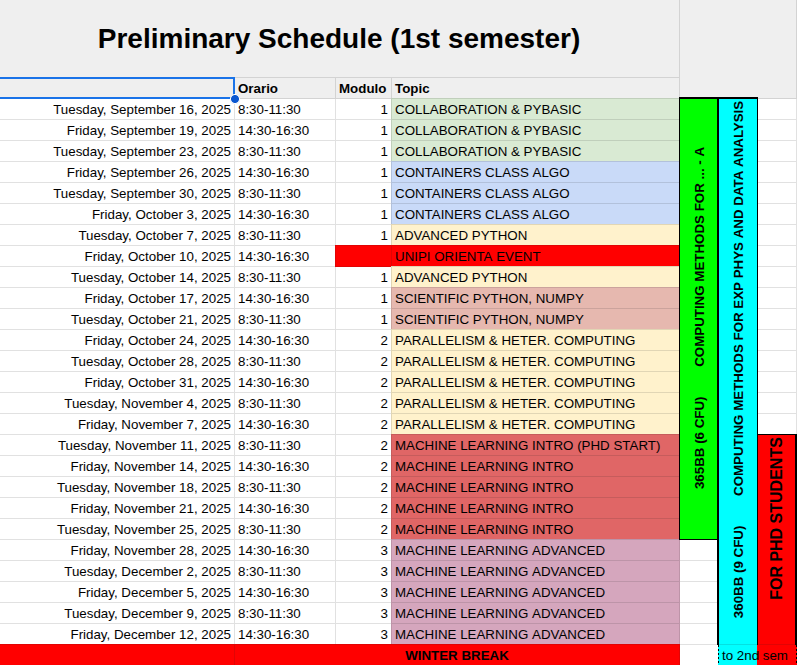
\includegraphics[width=0.8\textwidth]{figures/calendar_2025}
\end{frame}

\end{document}
